\chapter{Literature Survey}


\section {\textbf{ Bitcoin: A Peer-to-Peer Electronic Cash System}}
	\begin{figure}[!b]
	\centering
	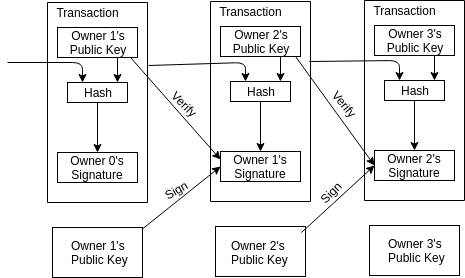
\includegraphics[width=\linewidth]{Images/BlockDiagramOfTransaction.png}
	\caption{Transactions}
	%\label{fig:universe}
\end{figure}
	      This paper focuses on a peer-to-peer version of electronic cash that would allow payments to be sent directly from one party to another without going through a financial institution and establishes the foundation of the technology used to achieve this objective i.e. Blockchain.
	      
        Today, transactions on the internet rely on financial institutions to process payments. The need for trusted third parties to mediate transactions makes non-reversible transactions impossible and increases the transaction costs. There is an acceptance that some fraud is inevitable. There is a need for an electronic payment system that uses cryptographic proof rather than trust and enables parties to transact with each other bypassing central third party.
	     
	    A Bitcoin is a chain of digital signatures. Every owner of an electronic coin passes it to the next owner by digitally signing: 
	    \begin{itemize}
	        \item A hash of the previous transaction
	        \item The public key of the new owner
	        \item Adding above 2 components to the end of the electronic coin
	    \end{itemize}
        
        A payee can verify the signatures to verify the chain of ownership. To avoid double spending of the coin without a trusted third party requires that transactions are declared publicly and all participants agree on a single history of the order in which they were received.
        
        
        The timestamp server takes the hash of a block of items, timestamps them and publicly publishes the hash. Each timestamp includes the previous timestamp, creating a chain, and as new timestamp hashes are added the chronological order and links are strengthened. Implementing a distributed time-stamp server requires a proof-of-work system.
        Proof-of-work requires scanning for a value which when hashed (e.g. using SHA-256) the hash value starts with a number of zero-bits. The average work required is exponential in the number of zero bits required. It Ensures that a verified block cannot be changed because all later blocks that are chained to it will also need to be changed (each subsequent block would need to be verified, requiring increasing CPU effort). It is based on a one-CPU-one-vote system, ensuring that the majority decision is based on the longest chain which requires the most proof-of-work effort.
	      
	     The steps to run the network are as follows:
	     \begin{itemize}
        \item New transactions are broadcast to all nodes.
        \item Each node collects new transactions into a block.
         \item Each node works on finding a difficult proof-of-work for its block.
        \item  When a node proof-of-work, it broadcasts the block to all nodes.
         \item Nodes accept the block only if all transactions in it are valid and not already spent.
        \item  Nodes express their acceptance of the block by working on creating the next bloc in the chain, using the hash of the accepted block as the previous block.   	     \end{itemize}
         The goal in peer-to-peer electronic cash system is to encourage nodes to connect to the network and validate transactions. The first block in a transaction starts a new coin which is owned by the creator of the block. In order to generate new blocks, and therefore coins (value), CPU and electricity are needed. If the output of a transaction is less than the input value, a transaction fee is added to the block containing the transaction.
         
Any old transactions can be removed to save disk space. To enable this removal without breaking the block hash value, transactions are hashed in a Merkle Tree. This allows for old blocks to be consolidated by essentially removing the tree branches, but keeping the root.

It is possible to verify payments without running a full network node. A user only needs to keep a copy of the block headers of the longest proof-of-work chain, which he can get by querying network nodes until he’s convinced he has the longest chain, and obtain the Merkle branch linking the transaction to the block it’s timestamped in. He can’t check the transaction for himself, but by linking it to a place in the chain, he can see that a network node has accepted it, and blocks added after it further confirm the network has accepted it. The verification is reliable as long as honest nodes control the network. To allow value to be divided and merged, transactions contain various inputs and outputs. For example, a single input from a large transaction, or many smaller inputs. 
Traditional banking limits access to information to just those involved in the transaction and the trusted third party. This is not workable in a model where the transactions are broadcast publicly, but the need for privacy is still important. Privacy is maintained by keeping public keys anonymous. A transfer can happen without knowing who is involved in the transaction. 

Where honest nodes control the majority of CPU power, a peer-to-peer network that uses proof-of-work to record public transactions makes it computationally impractical for attackers to tamper with.

\section {\textbf{ Legally Speaking: Smart Contracts,    Archival Bonds, and Linked Data in the Blockchain}}
	      This papers talks about the contract oriented programming language ‘Smart Contract'. It covers what is the language about and how to write it smart contracts.
	      	      
	      “Smart contracts,” in their purest form, seek to leverage the
	      trustless, immutable nature of the blockchain to empower peerto-peer,
	      disintermediated agreements enforced automatically
	      by code. Smart contracts, as such, are not legal contracts, but
	      rather, code to allow systems to execute a legal contract. 
	      
	      This paper explores
	      whether, by integrating language, by way of a semantic legal
	      layer, into blockchain-based smart contracts, smart contracts
	      could become full legal contracts. 
	      
	      The current blockchain landscape, in and of itself, is insufficient to capture the nuance of contract language, to preserve the evidence of the
	      contracting process for those cases where parol evidence might
	      be admissible, or to provide for the many non-financial terms
	      that parties typically negotiate as part of a contract. However,
	      the integration of a semantic legal layer – utilizing jurisdiction
	      specific legal ontologies – could add the precision, flexibility,
	      and enforceability to blockchain-based smart contracts to allow
	      them to serve the same purposes at their traditional progenitors. 
	      
	      
	      The great specificity and power of legal language necessitates that, if smart contracts are to have the flexibility and import of their traditional progenitors, smart contracts must be able to draw on
	      formal language of contract.
	      
	      Integrating legal language into smart contracting
	      processes, then, is no small feat. Particularly for contracts
	      between major enterprises, smart contracts are highly unlikely
	      to eliminate the need for legal counsel with expertise in both
	      the industry(ies) and jurisdiction(s) pertinent to the contract. A
	      number of clauses, such as choice of law, indemnification,
	      disclaimer of warranty, limit of liability, assignability,
	      termination, modification, and so forth, will still need to be
	      negotiated between parties. For contracting parties without
	      counsel at their disposal, however, fully legal smart contracts
	      could potentially “level the playing field,” giving them at least
	      some access, through an ontology, to the same language used
	      so effectively by attorneys, in addition to access to automated
	      enforcement. 
	      
	      Semantic Blockchain is a distributed database that maintains a continuously-growing list of standardized data records, using Resource Description Framework (RDF), hardened against tampering and
	      revision. Replace RDF with classification codes.
	      
	      Should one of the parties to a smart contract have issues with it after its formation or execution (for example, individuals who lost
	      money in the DAO hack), that party would first have to prove
	      the existence of a contract at all – a formidable feat for current
	      smart contracts, which can easily be made without a legal
	      contract coming into existence.
	      
	      While using linked data to help preserve the archival bond
	      in smart contracts offers a first step towards more enforceable
	      smart contracts, full blockchain-based legal contracts are
	      unlikely to happen without the integration of a legal ontology.
	      
	      The development of appropriate ontologies to support
	      full legal contracts on a semantic blockchain remains an open
	      challenge. While there exist a number of legal ontologies,
	      such LKIF-Core (an OWL ontology of “basic” legal
	      concepts), a great deal more granularity would be required to
	      properly support the use of smart contracts for full contracting
	      purposes. Furthermore, legal knowledge, despite the vast array
	      of code, cases, and statutes brought to bear, remains a largely
	      tacit affair.
	      
	      As Lemieux and Sporny assert, it is only by preserving the
	      archival bond that the unique identity of each record can be
	      preserved.“The archival bond contains within itself the
	      direction of the cause-effect relationship of the procedure
	      which gives rise to records, and it is therefore the primary
	      expression of the development of the activity in which the
	      document participates, rather than just facts about the act that
	      the document embodies.”Without the archival bond, it is
	      impossible to know if a contract has formed, because it is
	      impossible to reconstruct the relations of the records in such a
	      way as to prove that an “acceptance” was actually an
	      acceptance, as opposed to an attempt to accept a lapsed or
	      revoked offer. 
	      
	      The archival bond is also critical in cases where the
	      final reduction to writing of the contract between the parties is
	      only a partial integration of their understanding. In such a
	      case, “parol evidence,” or evidence beyond the four corners of
	      the contract, is admissible to prove the parties’ intentions
	      regarding terms beyond those captured in the contract. For
	      example, if the final contract doesn’t specify a time for
	      performance, parties can introduce evidence of their
	      negotiations regarding that term prior to the contract
	      formation. Without the archival bond, however, it becomes
	      impossible for the parties to clear the hurdles to admissibility
	      for documentary evidence, namely, the best evidence and
	      authenticity rules. Smart contract systems that don’t provide
	      for the archival bond leave any open terms largely to the
	      discretion of the courts.  
\section { \textbf{PBFT vs Proof-of-Authority: Applying the CAP Theorem to Permissioned Blockchain}}
	      	      
	      This paper introduces the concept of Proof of Authority consensus and how it is more efficient than the pBFT mechanism. It includes the Aura protocol, chain scoring and chain finality concepts. It also includes the comparison between Aura and pBFT.
	\begin{figure}[!h]
	\centering
	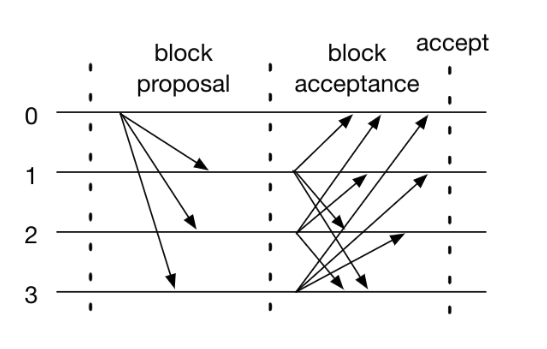
\includegraphics[width=\linewidth]{Images/aura.png}
	\caption{Transactions}
	%\label{fig:universe}
\end{figure}	      	      
	      Permissioned blockchains are arising as a solution to federate companies prompting accountable interactions. A variety of consensus algorithms for such blockchains have been proposed, each of which has different benefits and drawbacks. Proof-of-Authority (PoA) is a new family of Byzantine fault-tolerant (BFT) consensus algorithms largely used in practice to ensure better performance than traditional Practical Byzantine Fault Tolerance (PBFT). However, the lack of adequate analysis of PoA hinders any cautious evaluation of their effectiveness in real-world permissioned blockchains deployed over the Internet, hence on an eventually synchronous network experimenting Byzantine nodes. 
	      
	      In this paper, analysis of two of the main PoA algorithms, named Aura and Clique, both in terms of provided guarantees and performances. First, functionality is derived including how messages are exchanged, then weight, by relying on the CAP theorem, consistency, availability and partition tolerance guarantees. Reporting of a qualitative latency analysis based on message rounds is also done. The analysis advocates that PoA for permissioned blockchains, deployed over the Internet with Byzantine nodes, do not provide adequate consistency guarantees for scenarios where data integrity is essential but works well for large distributed platforms.
	      
	      Proof of Authority is a new family of BFT algorithms which has recently drawn attention due to the offered performance and toleration to faults. PoA requires less message exchanges hence provides better performance. PoA algorithms favour availability over consistency, oppositely to what PBFT guarantees. This can sometimes be not suitable for permissioned blockchains. PBFT can be a better choice but it can also be worse than some POA implementations. 
	      
	      PoA algorithms rely on a set of N trusted nodes called the authorities. Each authority is identified by a unique id and a majority of them is assumed honest, namely at least N/2 + 1. The authorities run a consensus to order the transactions issued by clients. Time is divided into steps, each of which has an authority elected as mining leader.The two PoA implementations work quite differently: both have a first round where the new block is proposed by the current leader (block proposal); then Aura requires a further round (block acceptance), while Clique does not.
	      
	      Aura : If authorities do not agree on the proposed block during the block acceptance, a voting is triggered to decide whether the current leader is malicious and then kick it out. An authority can vote the current leader malicious because (i) it has not proposed any block, (ii) it has proposed more blocks than expected, or (iii) it has proposed different blocks to different authorities.
	      
	      Clique: Clique computes the current step and related leader using a formula that combines the block number and the number of authorities. Each authority is only allowed to propose a block every N/2+ 1 blocks. 
	      
	      CAP Theorem : The CAP Theorem states that in a distributed data store only two out of the three following properties can be ensured: Consistency (C), Availability (A) and Partition Tolerance (P). Thus any distributed data store can be characterised on the basis of the (at most) two properties it can guarantee, either CA, CP or AP. 
	      \begin{itemize}
	      	\item A blockchain achieves consistency when forks are avoided.
	      	\item A blockchain is available if transactions submitted by clients are served and eventually     committed, i.e. permanently added to the chain.
	      	\item When a network partition occurs, authorities are divided into disjoint groups in such a way that nodes in different groups cannot communicate each other.
	      \end{itemize}
	      
	      By applying the CAP Theorem, it is claimed that in this setting PoA algorithms can give up consistency for availability when considering the presence of Byzantine nodes. PBFT keeps the blockchain consistent at the cost of availability, even when the network behaves temporarily asynchronously and Byzantine nodes are present; this behaviours is much more desirable when data integrity is a priority. 
	      	              
\section {\textbf{IPFS – Content Addressed, Versioned, P2P File System}}
	      	      
	      The paper introduces the concept of Inter-Planetary File system. It tells how the data is stored on IPFS servers and the data can be retrieved from those servers. It is the white paper of the IPFS technology.
	      	      
	      This paper introduces The InterPlanetary File System (IPFS), which is a peer-to-peer distributed file system that seeks to connect all computing devices with the same system of files. In some ways, IPFS is similar to the Web, but IPFS could be seen as a single BitTorrent swarm, exchanging objects within one Git repository. In other words, IPFS provides a high through-put content-addressed block storage model, with content-addressed hyperlinks. This forms a generalized Merkle DAG, a data structure upon which one can build versioned file systems, blockchains, and even a Permanent Web. IPFS combines a distributed hashtable, an incentive block exchange, and a self-certifying namespace. IPFS has no single point of failure, and nodes do not need to trust each other.
	      
	      Today, HTTP is the de-facto way to transmit files across the internet. It works pretty well to move small files because the process is cheap. But, HTTP fails to take advantage of new file distribution techniques invented in the past decade. The upgrades are nearly impossible without breaking backward compatibility and because of the huge investment in the current model of HTTP and the web. In the near future, there will be new challenges like:
	      Moving datasets in size of petabytes
	      High volume real-time media streams
	      Versioning and linking of massive datasets
	      Preventing accidental disappearance of important files
	      To understand how IPFS works, it is essential to understand what a Distributed Hash Table (DHT) is
	      A Hash Table is a data structure that represents an array of key-value pairs. It uses a hash function to compute an index/key. The hash table facilitates very fast lookup of values based on keys.
	      A Distributed Hash Table (DHT) is a distributed system that provides access to the key-value store. The store is spread over the participating nodes and offers excellent performance and scalability. DHTs are used widely in peer-to-peer system to coordinate and maintain metadata about the system.
	      
	      A NodeId identifies a node in the IPFS system. A NodeID is nothing but the hash of its public key. Nodes can change their NodeId anytime, but, they are incentivized to remain the same. The nodes store objects (of their interest) in their local storage. These objects represent files and other data structures in IPFS.
	      All nodes maintain a DHT that is used to find:
	      Network address of other peers in the network, and 
	      Peers who can serve a particular object
	      This DHT allows IPFS to find peers that can serve an object and be able to reach to the peer over the network.
	      IPFS uses a different content addressing method to identify content. This approach is different from what exists in the web today, where a server that contains the object addresses the content.
	      
	      IPFS content address resolves to an IPFS Object which contains a list of IPFS Links and some content data. When adding huge files to IPFS, it is broken into many smaller chunks, and the address resolves to a list of IPFS links that point to the chunks. This content addressing approach confirms that the address will always return the same file.
	      Another benefit of this approach is that as long as one of the nodes has the content, it can always be accessed from the IPFS network. This solves the dead-link problem that exists in today’s internet. Duplicate files do not take multiple of space because it will always point to the same content hash. Having just one copy in the network is enough for it to be retrievable from the network.
	      
	      Given the content address, the IPFS network responds with the peers that have the required objects. The object and its links can be received simultaneously from multiple peers.
	      Our peers can share the object after IPFS returns it from the network. The node can also verify that the content has not been tampered with because hash value maps to content in the IPFS network. Since the content of the file generates the content address (hash), it changes whenever a file is modified.
	      It is not convenient to share a new content address every time the file changes. To tackle this issue, IPFS has a concept of IPNS, or the Inter Planetary Name System.
	      IPFS provides a generic way to share files and data in a peer to peer fashion optimizing delivery. Some of the use case scenarios where IPFS would be great are:
	      Sharing files and huge datasets.
	      Serving websites and blogs on IPFS.
	      Using as a data source or sink in data processing workflows.
	      Using as a Mounted filesystem.
	      
	      The white-paper discusses a peer-to-peer, version-controlled approach to a filesystem. This filesystem has no single point of failure. Since the data is content-addressed, the nodes in the network don’t need to trust each other. As per this paper, IPFS has the potential to replace HTTP and make the web, distributed.
	    
